%%%%%%%%%%%%%%%%%%%%%%%%%%%%%%%%%%%%%%%%%%%%%%%%%%%%%%%%%%%%
% Template prepared by Dr Daniel Oi, CC BY-NC 4.0          %
%%%%%%%%%%%%%%%%Do Not Alter The Preamble%%%%%%%%%%%%%%%%%%%

%%%%%%%%%%%%%%% Preamble Starts Here %%%%%%%%%%%%%%%%%%%%%%%
%
\documentclass[aps,pra,a4paper,nofootinbib,onecolumn,tightenlines,longbibliography,12pt,amsfonts,amssymb,amsmath,floatfix]{revtex4-2} % Uses the APS RevTeX document class. Versions earlier than 4-2e may not be compatible with the latest LaTeX kernel.
\usepackage{latexsym,graphicx,color,geometry}
\geometry{a4paper, portrait, hmargin=2cm, vmargin={2cm, 2.5cm}}%Defines the page size and margins
\usepackage{url}%Fixes URLs in bibliography
\usepackage{enumitem}%Numbering in Lists
\usepackage[english]{isodate,babel}
\usepackage[figure,table]{totalcount} % counts tables and figures
\usepackage{blindtext} % used to make some example junk text
\usepackage{physics} % very useful for typesetting physics equations
\usepackage{float}
\def\bibsection{\section*{\refname}} %Sorts out reference section and gets rid of horizontal line
\bibliographystyle{acm}
\usepackage{titlesec}
\titleformat*{\section}{\Large\bfseries}
\titleformat*{\subsection}{\large\bfseries}
\titleformat*{\subsubsection}{\normalsize\bfseries\itshape}
\titleformat*{\paragraph}{\large\bfseries}
\titleformat*{\subparagraph}{\large\bfseries}

%%%%Font Definition%%%%
% the document is to be sans serif
\usepackage[T1]{fontenc}
%\usepackage[cmbright]{sfmath}
\usepackage{lmodern}
\renewcommand{\rmdefault}{lmss}
\renewcommand{\sfdefault}{lmss}
\renewcommand{\mathbf}[1]{\ensuremath\textbf{\textit{\textsf{#1}}}}

%%%%%%%%%%%%%%%%%%% Preamble Ends Here %%%%%%%%%%%%%%%%%%%%%%%%


%%%%%%%%%%%%%%%%%%%%%%%%%%%%%%%%%%%%%%%%%%%%%%%%%%%%%%%%%%%%%%%
% Insert any other extra packages or definitions you want here%


%                                                             %
%%%%%%%%%%%%%%%%%%%%%%%%%%%%%%%%%%%%%%%%%%%%%%%%%%%%%%%%%%%%%%%


%%%%%%%%% Fill in your details in the part below %%%%%%%%%
\newcommand{\projecttitle}{Evaluating Spot Finding Methods}% Change title and remove red text color
\newcommand{\studentname}{Anton Gashi}% Type in your name here, but without the red highlighting, same for all other uses of red text
\newcommand{\regnumber}{201914462}
\newcommand{\degree}{MPhys}
\newcommand{\primarysup}{Dr Sebastian Van De Linde}
\newcommand{\secondsup}{Dr Daniel Oi}%Comment out this line if not needed
%\newcommand{\thirdsup}{\textcolor{red}{Dr~C~Bloggs}}%Comment out this line if not needed
%%%%%%%%%%%%%%%%%%%%%%%%%%%%%%%%%%%%%%%%%%%%%%



%%%%% Do Not Alter this part %%%%%%%%%%%%
\usepackage{fancyhdr}
\pagestyle{fancy}
\setlength{\headheight}{14pt}
\footskip = 45pt
\fancyhf{}
\lhead{\projecttitle} 
\lfoot{PH450 Report 2021-22}
\cfoot{Student: \regnumber}
\rfoot{Page \thepage}
%%%%%%%%%%%%%%%%%%%%%%%%%%%%%%%%%%%%%%%%%


%%%%%%The document starts here%%%%%%
\begin{document}

%%This section creates the cover page%%

\begin{figure}
\includegraphics[width=\textwidth]{ScienceLogo.png}
\end{figure}

\title{PH450 Report 2021-22\\ \vspace{1cm}
{\huge \projecttitle}\\[0.5cm] %If your title is too long, use \LARGE, \Large, or large instead of \huge
{\footnotesize Submitted in partial fulfilment for the degree of \degree}}

\author{\studentname\\
Registration No.: \regnumber}
\affiliation{SUPA Department of Physics, University of Strathclyde, Glasgow G4 0NG, United Kingdom}

\author{\primarysup{} (Primary Supervisor)}
\noaffiliation
\ifdefined\secondsup % this only appears if \secondsup is set above
\author{\secondsup, (Secondary Supervisor)} % 
\noaffiliation
\fi
\ifdefined\thirdsup
\author{\thirdsup, (Secondary Supervisor)} % 
\noaffiliation
\fi

\date{\today}

\pagenumbering{gobble} % first page in document is not numbered

\maketitle
%%This ends the title page section%%

\newpage % Creates a new page

\pagenumbering{roman} %Use Roman numerals for the front matter pages

\section*{Abstract} %The * suppresses a section number
\addcontentsline{toc}{section}{Abstract}

\newpage
\section*{Acknowledgements}
\addcontentsline{toc}{section}{Acknowledgements}


%%%%%%%%%%%%%%%%%%%%%%%%%%%%%
% Do not alter this section %
\newpage
\tableofcontents % Creates a Table of Contents
\makeatletter
\let\toc@pre\relax
\let\toc@post\relax
\makeatother

\ifnum\totalfigures>0
\newpage
\listoffigures
\addcontentsline{toc}{section}{List of Figures}
\fi

\ifnum\totaltables>0
\newpage
\listoftables
\addcontentsline{toc}{section}{List of Tables}
\fi


% Can edit after here       %
%%%%%%%%%%%%%%%%%%%%%%%%%%%%%


%%%%% Main Report Starts Here %%%%%

\newpage
\pagenumbering{arabic}

\section{Introduction}

  \subsection{Sub-Pixel Localisation} % (fold)
  \label{sub:spot-finding intro}
  
  Super-resolution microscopy is the process of taking the diffraction limit 
  of a microscope, ~250nm in the x and y direction, and improving it at a minimum by a 
  factor of 2 although more modern methods improve it by up to a factor of 10. In the past this has been achieved by ensemble techniques
  like SIM (Structured Illumination Microscopy) and STED (Stimulated Emission Depletion)
  \textbf{insert explanation of ensemble techniques}. An improvement on these methods 
  is single-molecule microscopy, in which molecules are individually fluoresced and 
  imaged instead of ensembles which helps distinguish more detail and produce better
  results than the diffraction limit.
  There are two ways that this general method have been implemented; photo-activated localization
  microscopy(PALM) and stochastic optical reconstruction microscopy(STORM), both
  rely on fluorophores which are fluorescent chemicals that re-emit light after
  being excited. This helps as the fluorescence emits the light 
  stochastically so only a subset of molecules "light-up" at once, this is important 
  as if they are separated by at least 200nm then they can be located to nanometre precision. 
  Since the molecules are now separated spatially this process needs to just needs to be repeated 
  until all molecules have been "switched-on", this gives a stack of images with blurry spots
  which can be located and recombined into a final image with spot-precision on the order of <~20nm.\cite{galbraith2011super}
  The resolution of a super-resolution image usually doesn't refer to the spot-precision of the 
  located molecule, rather it refers to the structural resolution, this can be calculated along 
  with the density of fluorophores as the Nyquist-Shannon sampling theorem states a minimum number 
  of fluorophores are required to resolve the structure. For example if the resolution is 20nm in 
  one dimension then fluorophores have to be separated at least 10nm apart at a density of 
  $~10^4\mu m^{-2}$.\cite{van2011single}\cite{shannon1949communication}

  \subsubsection{Pixels and Resolution} % (fold)
  \label{ssub:Pixel}
   In the Modern Dictionary of Electronics by Graf a pixel is described as a, 
   spatial resolution element.
   The smallest distinguishable and resolvable area in an image.
   \cite{graf1997modern}
   This was mainly in reference to an analog image but the principle applies 
   to a raster image, which is a NxM matrix of values that display colour and
   intensity. In the specific case of the spot localisation that the Methods section 
   (\ref{sec:Methods}) describe the images are NxN and 16-bit black and white.

   Resolution is the capability of resolving two points or lines.
   Since super-resolution by definition changes the resolution of the input images, 
   the resolution of the output image needs to be quantified.
   One of the ways to do this is by using the Nyquist-Shannon sampling theorem,
   this states that \textbf{fix reference in bib file->}\cite{DEMPSEY2013561}\cite{tinnefeld2015far}
  % subsubsection Pixel (end)

  
  \subsection{Motivation} % (fold)
  \label{sub:Motivation}
  
  The main motivation behind my project is to improve the compute time that it
  takes to render images through sub-pixel localisation whilst keeping an
  acceptable level of accuracy. That is to say this project should be aiming to
  produce a method of spot-finding that either less complex, less computations
  per localisation, fewer steps or a mixture of all. 

  This doesn't just have applications in localisation microscopy but also 
  can be used in other technologies, for example a paper published by Castorena and Creusere \cite{6638050}
  has the problem of needing a fast super-resolution technique to get higher 
  spatial resolution from their LIDAR (Light Detection and Ranging) system. This system is constrained by the 
  laser spot size and precision of the scanning mechanical unit as the single laser 
  source with sampling rates in the GHz range which achieves high accuracy for depth 
  and range resolution but poor spatial resolution. A consideration was to decrease the 
  diameter of the laser thus increasing the spatial sampling density, although this 
  was deemed too computationally expensive.
  
  With the almost exponentially increasing launching of small form factor
  satellites such as the CubeSat, arises the challenge of efficiently utilising
  the satellites computing resources. This means any segment of code being ran on
  the satellite needs to run as quickly as possible whilst keeping a certain
  standard of accuracy, especially for the processes that the satellite depends
  on to operate like attitude control, power management and calculations for
  orbital maneuvers. The main method used for orienting(attitude control) CubSat
  like satellites is by using a Star Tracker, this works by using a camera mounted
  facing stars that are known to the satellite via a star catalogue and moves
  based on how aligned or unaligned a reference image is with the actual image
  seen.\cite{calitz2015design} The method in which the image is processed so it
  can be compared to the reference is called spot finding, this entails taking
  the image and finding each bright spot or star accurately. The motivation for
  this project is to develop a spot finding method for star tracking and compare
  it to the state of the art algorithms measuring accuracy, precision and speed.

  This technique is also used for super-resolution microscopy, which changes the
  optical limits of microscopy from 250nm to about 10nm, this is achieved by
  temporally or spatially spacing the light coming from the specimen being
  imaged. 

  \textbf{still need to add more technologies that use spot localisation}
  
  \subsection{Literature Review (don't call it literature review)} % (fold)
  \label{sub:Literature Review (don't call it literature review)}
  
  % subsection subsection name (end)

% subsection subsection name (end)


\section{Literature Review} % (fold)
\label{sec:lit review}


The field of spot finding or star finding is a fairly recent field with papers
coming out in the mid 80's from NASA. However the methods haven't changed that
much since the main algorithm still used is centroiding since it's a very good
compromise between quickness and accuracy being that it can give an answer in
the 1-100 microsecond range \cite{delabie2014accurate}. Much of the innovation
has come from optimising the algorithm or optimising the data going into the
algorithm. 


\section{Methods} % (fold)
\label{sec:Methods}

  \subsection{Centroiding} % (fold)
  \label{sub:Centroiding_meth}
  
  % subsection subsection name (end)
  
  
  The most common way of spot finding for star tracking is to use centroiding
  algorithms, this is when a subsection of pixels are considered to be a star
  using a rough calculation. The area of interest is then filtered in such a way
  that reduces noise and aberrations, finally apply the algorithm in this case
  it's the center of gravity method (\ref{eq1})(or the moment
  method)\cite{delabie2014accurate}\cite{stone1989comparison}.
  \begin{equation}\label{eq1}
      (x_b,y_b) = \left( {\frac{\sum_{ij} I_{ij}x_{ij}}{\sum_{ij} I_{ij}},\frac{\sum_{ij} I_{ij}y_{ij}}{\sum_{ij} I_{ij}}}\right)
  \end{equation}
  
  As can be seen in equation \ref{eq1} the centroiding method is fairly trivial, 
  the part that determines the computational operations needed is the i and j terms. 
  These terms are the 'window' of pixels that have been chosen by another rough estimator 
  to get a generalised position, the window is a square around the estimated position so 
  the computation scales like $n^2$, where n is the window size.\cite{stone1989comparison}
  
  \subsection{Fitting methods} % (fold)
  \label{sub:Various fitting methods}

  \subsubsection{Point Spread Function} % (fold)
    \label{ssub:Point Spread Function}
    
    Point Spread Functions(PSF) is the way an object blurs due to the imaging of a point 
    source of light, it's the reason the diffraction limit of a microscope is 250nm (in the
    x,y direction) and >450-700nm (in the z direction).\cite{galbraith2011super} The PSF is also the smallest resolvable
    detail that can be seen with light as other objects that emit light that are smaller than 
    one another all appear to be the same size. Provided that laboratory equipment is set up correctly, 
    i.e. the lens is corrected for aberrations and constants are known such as aperture and angels 
    between lens and samples, methods like the Richards-Wolf model and Gibson-Lanni model will calculate
    the centre of a spot near perfectly. The problem with these methods is that they are complicated and 
    slow, and also offer an answer that is unnecessarily accurate. \cite{richards1959electromagnetic}\cite{small2014fluorophore}


    % subsubsection Point Spread Function (end)
    \subsubsection{Gaussian} % (fold)
    \label{ssub:Gaussian}

    Where the exact prediction of section (\ref{ssub:Point Spread Function}) fails Gaussian fitting tries to succeed 
    by presuming that, if all equipment is set up correctly, the centre of a PSF of a point source is 
    always going to be in the centre. Thus for 2-D spot finding that can't afford the computational time of 
    the previous method uses the more simple equation:

    $$I(x,y)=I_0\cdot \exp(-a\cdot k^2((x-x_0)^2+(y-y_0)^2))+b$$

    Where k is $\frac{2\pi}{\lambda}$, $a$ is the width of the PSF, $I_0$ is the peak intensity and b is the average background per pixel. \cite{small2014fluorophore}

    
    \subsubsection{Triangular method} % (fold)
    \label{ssub:Triangular method}
    
    The triangle method being used takes inspiration from the Gaussian method, in which,
    a Gaussian curve is produced and the area is calculated by integrating the function. 
    After this the position of the spot is estimated by a hyper-parameter optimisation method 
    which minimises the residual area left over from the fitting process.
    This triangle method looks to reduce the computational load by removing the integration step, 
    this can be done as the area of a triangle is just $\frac{1}{2}\ base\cdot height$. 
    On top of this, the method also sums pixel intensities across axis, firstly it gives a 
    better signal to noise ratio but also it means the triangle only needs to be rendered in 2 dimensions 
    instead of 3, further reducing the computational time. 

    \begin{figure}[H]
      \begin{center}
        \includegraphics[width=0.6\textwidth]{project_pics/visual_test_2.png}
      \end{center}
      \caption{Graph of ideal spot data}
      \label{fig:visual_test_2}
    \end{figure}

    \begin{figure}[H]
      \begin{center}
        \includegraphics[width=0.6\textwidth]{project_pics/visual_test.png}
      \end{center}
      \caption{Graph of data from figure \ref{fig:visual_test_2} with the calculated area and residual}
      \label{fig:visual_test}
    \end{figure}
    
    As can be seen in figure \ref{fig:visual_test} the area of the simulated spot are subtracted from 
    the area under the triangle and a residual is left over, this residual parameter is the 
    variable to be minimised for in the optimisation routine.

    \begin{figure}[h]
      \begin{center}
        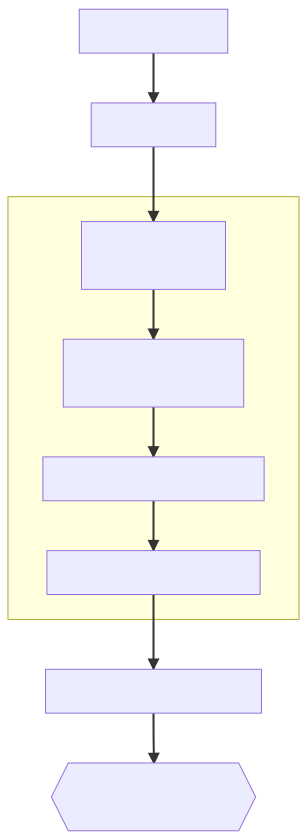
\includegraphics[width=0.4\textwidth]{project_pics/flowchart.png}
      \end{center}
      \caption{Flowchart describing how the code for the triangular fitting method works}
      \label{fig:flowchart}
    \end{figure}
    
    
    

\section{Results and analysis} % (fold)
\label{sec:Results}

  \subsection{Centroiding} % (fold)
  \label{sub:Centroiding_results}
  
  \subsection{Triangle Fitting} % (fold)
  \label{sub:Triangle Fitting}

  In figure \ref{fig:single_test} it can be seen that while using simulated data the mean accuracy of the 
  localisation is ~0.4 of a pixel whilst being executed in ~0.34s.

  \begin{figure}[H]
      \begin{center}
        \includegraphics[width=0.7\textwidth]{project_pics/single_test.png}
      \end{center}
      \caption{Simulated spots with R1.00, A: Error in the X direction, B: Error in the Y direction, C: Absolute error from the ground-truth}
      \label{fig:single_test}
    \end{figure}


    Part C of figure \ref{fig:single_test} has been replicated for all simulated spots given in figure \ref{fig:no_noise_all_r}
    to compare how the change in spot size changes accuracy.

  \begin{figure}[H]
    \begin{center}
      \includegraphics[width=0.7\textwidth]{project_pics/no_noise_all_r.png}
    \end{center}
    \caption{Spot localisation (like graph C in figure \ref{fig:single_test}) of different radii, R, on perfect data (executed in 2.4s)}
    \label{fig:no_noise_all_r}
  \end{figure}
  
  
  \begin{figure}[H]
    \begin{center}
      \includegraphics[width=0.7\textwidth]{project_pics/single_histo.png}
    \end{center}
    \caption{A: Absolute error from the ground-truth for R1.00, B: A histogram of errors from graph A}
    \label{fig:single_histo}
  \end{figure}
  

  \begin{figure}[H]
    \begin{center}
      \includegraphics[width=0.7\textwidth]{project_pics/distro.png}
    \end{center}
    \caption{Histograms of the absolute error from each radii}
    \label{fig:distro}
  \end{figure}


\begin{table}[H]
\begin{center}
\begin{tabular}{||c || c c||} 
 \hline
 Radii & Average & Variance \\ [0.5ex] 
 \hline\hline
 1.00 &  0.3850& 0.0177 \\ 
 \hline  
 1.41 &  0.3850& 0.0177  \\
 \hline 
 2.00 &  0.3850& 0.0177 \\
 \hline 
 2.83 &  0.3850& 0.0177 \\
 \hline 
 4.00 &  0.3850&  0.0177 \\ 
 \hline 
 5.66 &  0.3850& 0.0177 \\
 \hline
 8.00 &  0.3847& 0.0189\\ [1ex] 
 \hline
\end{tabular}
\end{center}
\caption{Values of figure \ref{fig:distro}}
\label{table1}
\end{table}
 
Figures \ref{fig:single_histo} \& \ref{fig:distro} and Table \ref{table1} are a demonstration of how the absolute
error of the spots are in a general Gaussian or normal distribution. 
  
  
      

\section{Discussion} % (fold)
\label{sec:Discussion}


  \subsection{Results in context of my aims} % (fold)
  \label{sub:Results in context of my aims}

  \subsection{Results in comparison with other studies/industry standard} % (fold)
  \label{sub:Results in comparison with other studies/industry standard}
  
  \subsection{Explanations for unexpected results} % (fold)
  \label{sub:Explanations for unexpected results}
  
  \subsection{Discuss improvements} % (fold)
  \label{sub:Discuss improvement}

% subsection subsection name (end)


\section{Conclusion} % (fold)
\label{sec:Conclusion}

% section :Conclusion (end)


\bibliographystyle{unsrt}
\bibliography{myreferences}%reads a .bib file called myreferences.bib for the actual references in BibTeX format. You can call your BibTeX file something else if you prefer.
\addcontentsline{toc}{section}{References}
%If there are problems with compiling the LaTeX file with BibTeX, make sure that file names don't have spaces in them as this might cause problems


% If there are appendices, these starts from here. Remove from this line until just before \end{document} if you are not using it 

\end{document}
